\chapter{Extensive air shower parameters estimation}

\section{Shower photon packets}
\label{sec:signal-reconstruction}

After deconvolution, our goal is to identify EAS photons among the background. These photons are expected to arrive in "packets" with a normal distribution of arrival times, characterized by parameters $n_{EAS}$ (total number of photons), $\mu_t$ (mean arrival time), and $\sigma_t$ (arrival time standard deviation). The background, composed of starlight and zodiacal light reflected from the snow, follows a Poisson distribution with mean $\lambda_{n}$ known from calibration.

We approach this as a Bayesian problem, seeking the posterior distribution of EAS photon packet parameters based on the distribution for $\vec{n}$ obtained from deconvolution.

The likelihood function is calculated by sampling signal, subtracting it from the $\vec{n}$ and calculating Poisson likelihood for the remaining background signal.

After that, we use similar MCMC technique to get the final signal reconstruction result: posterior distribution of photon packet parameters. Performing both steps of the analysis within the same Bayesian framework lets us effectively chain these two analysis together, while also keeping them separate.

We can also use Bayesian information criterion (BIC) \cite{Schwarz1978} to calculate the significance of EAS signal in each channel. We use it to remove background-only channels from further analysis.

Figure \ref{pic:deconvolution-and-reconstruction} shows an example of full EAS photon packet parameters reconstruction for an experimental event.

\begin{figure}
	\centering
	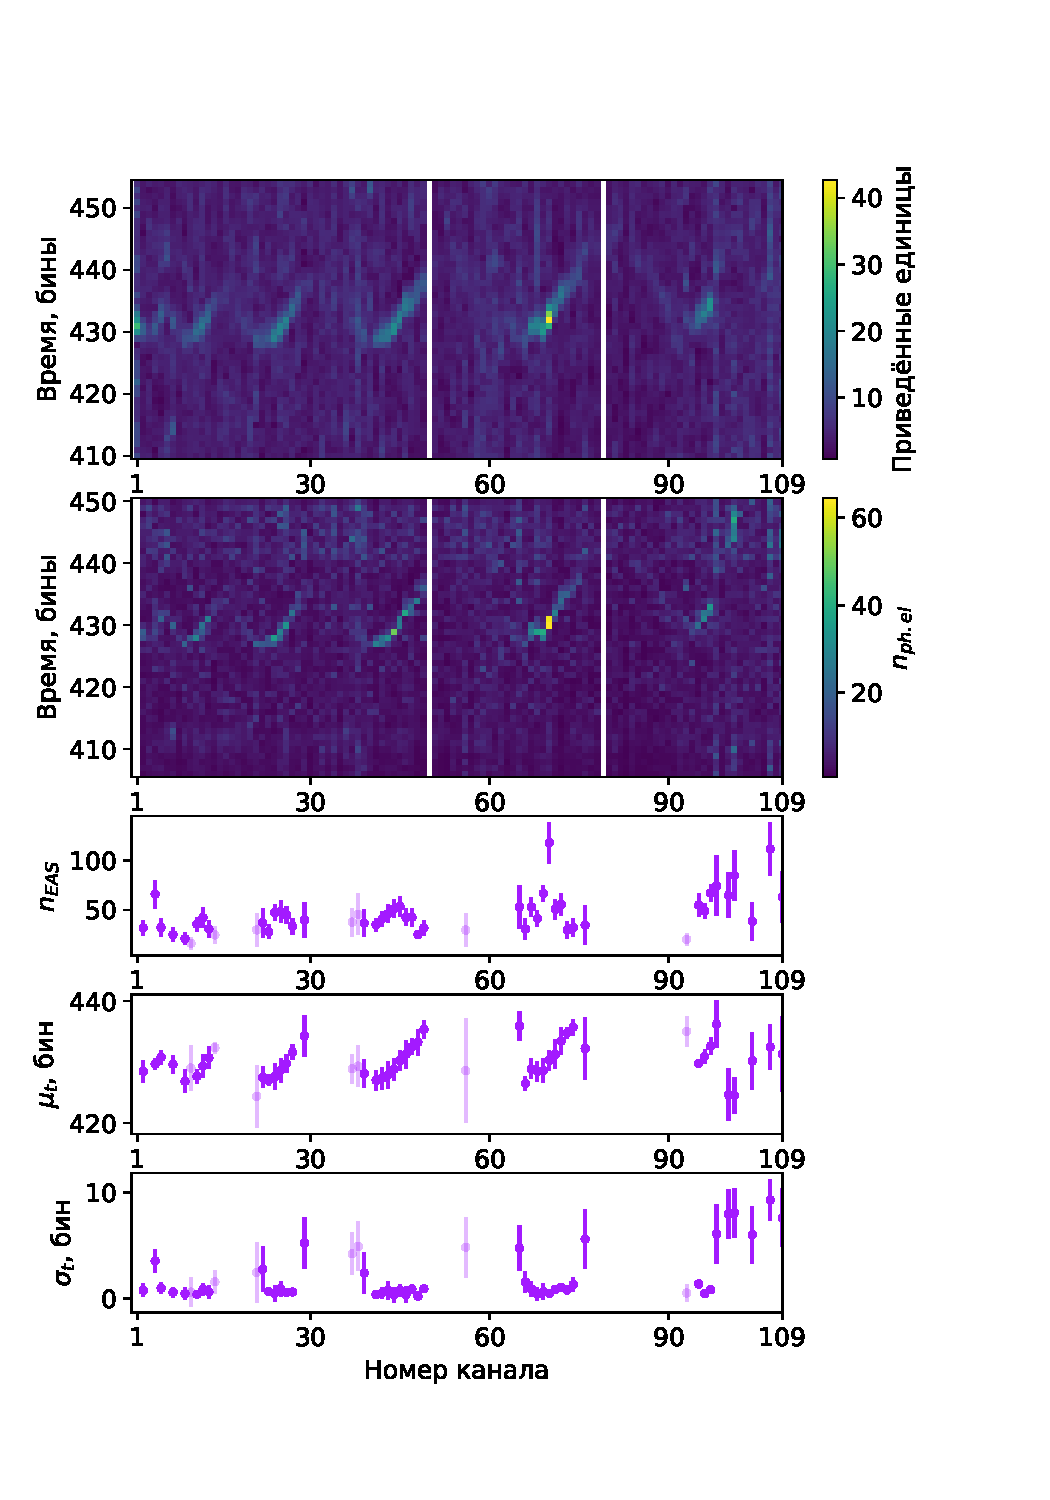
\includegraphics[width=0.86\columnwidth]{deconvolution-and-reconstruction}
	\caption{Full signal reconstruction for experimental event \#10675. Common X axis: channel number, see \cite{SphereCalibration2016} for numbering scheme. Top panel: experimental data with calibration coefficiens applied. Second-to-top panel: deconvolution output, photon count in each time bin. Three bottom panels: reconstructed photon packet parameters $n_{EAS}, \mu_t, \sigma_t$ --- dots and error bars represent marginal means and standard deviations; dimmed values are signals with $\Delta \mathrm{BIC} \in (0, 4]$, negative $\Delta \mathrm{BIC}$ (background-only channels) are omitted.}
	\label{pic:deconvolution-and-reconstruction}
\end{figure}


\section{Shower parameter reconstruction}

The rest of the reconstruction performed here in this work standard methods, with the exception of being applied to the output of Bayesian reconstruction.

\begin{itemize}
	\item \textbf{Shower arrival direction} is determined by a plain fit of arrival times. Ground level arrival times for each channel are determined from $\mu_t$ by subtracting ground-to-detector light travel time, accounting for the detector altitude and inclination.
	\item \textbf{Shower axis position} is determined by finding a point on the surface that maximizes the probability (with respect to each channel's posterior distribution) of monotonously decreasing lateral distribution function.
	\item \textbf{Lateral distribution function} for EAS Cherenkov light is determined by fitting a parametrized function to the data. In  this work, a simplified LDF from \cite{Budnev2005} is used. The fitting is done by convolving the LDF with each channel's light collection function (which is calculate from detector's optic system model). Shower energy is then derived from LDF parameters.
\end{itemize}
